\documentclass{standalone}

\usepackage[OT1]{fontenc}
\renewcommand*\familydefault{\sfdefault}
\usepackage{helvet,sfmath}
\usepackage{siunitx}

\usepackage{tikz}
\usetikzlibrary{arrows,calc,patterns}
% \usetikzlibrary{intersections, calc, arrows.meta}
\usepackage{tikz,tkz-euclide}

\begin{document}
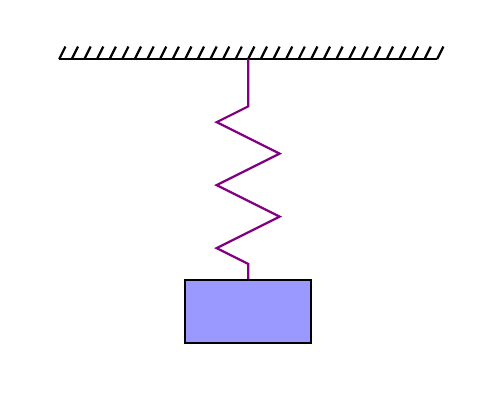
\begin{tikzpicture}[scale=0.8, >=Stealth]

    %% Background
    \draw[draw=none] (-3.5,0.5) rectangle (3.5,-5);

    \draw[thick] (-3,0) to (3,0);

    \foreach \x in {-3,-2.8,...,2.8,3}
    {
    \draw[thick] (\x,0) to (\x+0.1,0.2);
    }

    \draw[thick, violet] (0,0) to (0,-0.75) to (-0.5,-1) to (0.5,-1.5) to (-0.5,-2) to (0.5,-2.5) to (-0.5,-3) to (0,-3.25) to (0,-3.5);

    \draw[thick, fill=blue!40] (-1,-3.5) rectangle (1,-4.5);
    
\end{tikzpicture}
\end{document}